%!TEX ROOT = thesis.tex
\chapter{LITERATURE REVIEW}
\label{chapter: 2}

This chapter would cover the literature review part of this project. The first section would elaborate on the datasets evaluated, including the data exploratory analysis of the datasets.  The second and third sections would include a brief introduction to traditional methods semantic segmentation and their limitations respectively. The fourth sections would serve as a literature review of semantic segmentation using Convolutional Neural Networks. The fifth and last section would include the literature review of semantic segmentation using transformers and its advantages.

\section{Satellite Images Datasets}

\FloatBarrier
\begin{table}[]
\begin{tabular}{|c|c|c|c|c|c|c|}
\hline
\textbf{Dataset}                                                      & \textbf{Source}                                                & \textbf{\# Samples} & \textbf{\# Classes} & \textbf{Size (px)} & \textbf{Res (m)} & \textbf{Band}                                      \\ \hline
\begin{tabular}[c]{@{}c@{}}Benin Cashew \\ Plantation\end{tabular}    & Airbus Pléiades                                                & 70                  & 6                   & 1,122x1,186        & 10               & MSI                                                \\ \hline
\begin{tabular}[c]{@{}c@{}}Cloud Cover \\ Detection\end{tabular}      & Sentinel-2                                                     & 22,728              & 2                   & 512x512            & 10               & MSI                                                \\ \hline
\begin{tabular}[c]{@{}c@{}}Kenya Crop \\ Trade\end{tabular}           & Sentinel-2                                                     & 4,688               & 7                   & 3,035x2,016        & 10               & MSI                                                \\ \hline
\begin{tabular}[c]{@{}c@{}}Deep Globe \\ Land Cover\end{tabular}      & \begin{tabular}[c]{@{}c@{}}DigitalGlobe\\  +Vivid\end{tabular} & 803                 & 7                   & 2,448x2,448        & 0.5              & RGB                                                \\ \hline
DFC2022                                                               & Aerial                                                         & 3,981               & 15                  & 2,000x2,000        & 0.5              & RGB                                                \\ \hline
\begin{tabular}[c]{@{}c@{}}ETCI 2021 \\ Flood Prediction\end{tabular} & Sentinel-1                                                     & 66,810              & 2                   & 256x256            & 5–20             & SAR                                                \\ \hline
\textbf{GID-15}                                                                & Gaofen-2                                                       & 150                 & 15                  & 6,800x7,200        & 3                & RGB                                                \\ \hline
\textbf{LandCover.ai}                                                          & Aerial                                                         & 10,674              & 5                   & 512x512            & 0.25–0.5         & RGB                                                \\ \hline
\textbf{LoveDA}                                                                & Google Earth                                                   & 5,987               & 7                   & 1,024x1,024        & 0.3              & RGB                                                \\ \hline
\textbf{Potsdam}                                                               & Aerial                                                         & 38                  & 6                   & 4,000x4,000        & 0.02             & RGB                                                \\ \hline
\textbf{Vaihingen}                                                             & Aerial                                                         & 33                  & 6                   & 1,281–3,816        & 0.09             & RGB                                                \\ \hline
SEN12MS                                                               & \begin{tabular}[c]{@{}c@{}}Sentinel-1/2, \\ MODIS\end{tabular} & 180,662             & 33                  & 256x256            & 10               & \begin{tabular}[c]{@{}c@{}}SAR,\\ MSI\end{tabular} \\ \hline
\end{tabular}
\caption{Datasets for Semantic Segmentation Task}
\label{tab:datasets}
\end{table}

\FloatBarrier

Table \ref{tab:datasets} shows the list of dataset that were evaluated and considered for this project. Each of the dataset is made for semantic segmentation task and  is provided by the TorchGeo library. The dataset in bold are the ones that I think deserve more in depth exploration and discussion. 

%%Potsdam%%%
The Potsdam and Vaihingen datasets \cite{potsdam-vaihingen} are datasets made specifically for urban semantic segmentation used in the 2D Semantic Labeling Contest - Potsdam and 2D Semantic Labeling Contest - Vaihingen respectively. Both of the datasets are available upon request \href{https://www.isprs.org/education/benchmarks/UrbanSemLab/detection-and-reconstruction.aspx#VaihigenDataDescr}{here}. Although the images are not taken by satellites, a lot of literature reviewed such as \cite{unetformer}, \cite{a-novel-transformer}, \cite{multi-attention-network} and \cite{A2-FPN} train their semantic segmentation model using these datasets thus we think these merit a bit of discussions. Vaihingen dataset is composed of 33 orthorectified image tiles acquired by a near NIR-RGB drone camera, over the town of Vaihingen, Germany. The average size of the images is 20494 x 20064 pixels with a spatial resolution of 9 cm. Potsdam dataset is composed of 38 orthorectified image tiles acquired  over the town of Potsdam using the same NIR-RGB drone camera.. The average size of the tiles is also 20494 x 20064 pixels but with a smaller spatial resolution of 5 cm. Images in both datasets are accompanied by a digital surface model (DSM) representing the absolute height of pixels. There are a total of 6 classes in each dataset:

\begin{enumerate}
    \item Impervious Surfaces - roads, concrete surfaces 
    \item Buildings 
    \item Low Vegetation 
    \item Trees 
    \item Cars  
    \item Clutter - representing uncategorizable land covers
\end{enumerate}

\FloatBarrier
 \begin{figure}[ht]
\includegraphics[width=11.5cm, height=7cm]{images/potsdam-image.png}
\centering
\caption{An Image From Potsdam Dataset}
\label{fig:potsdam-image}
\end{figure}

\begin{figure}[ht]
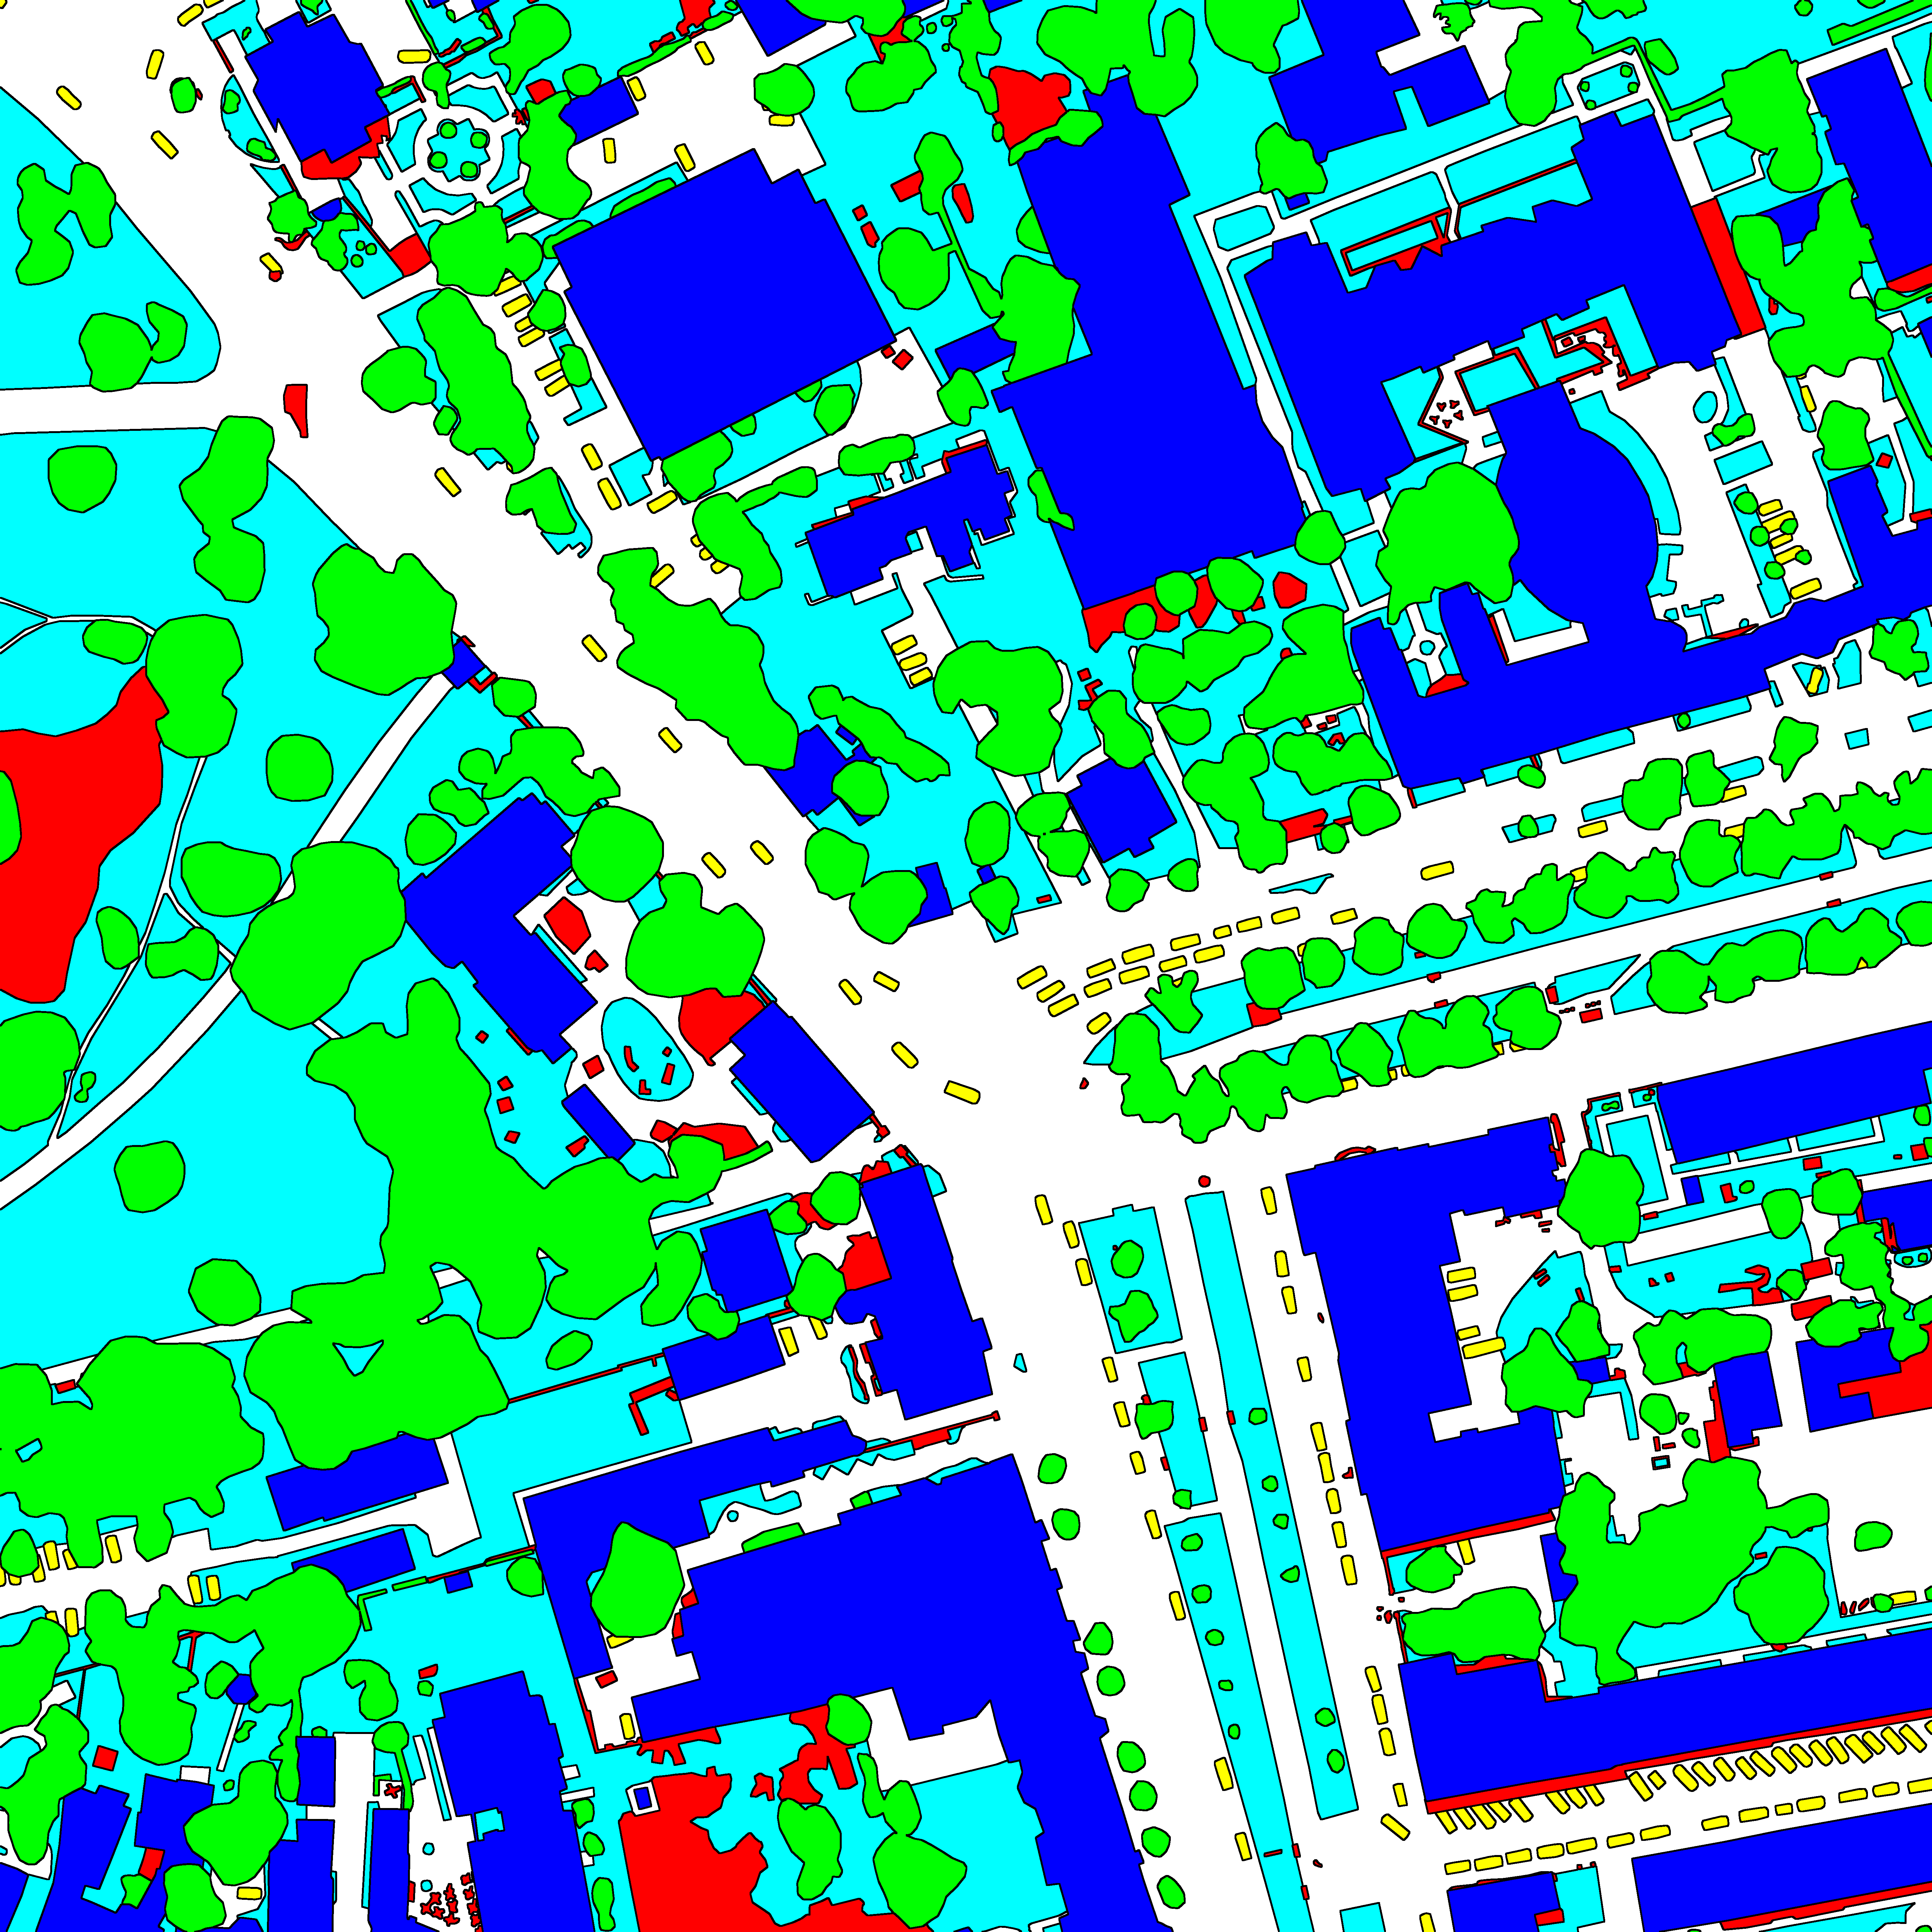
\includegraphics[width=11.5cm, height=7cm]{images/potsdam-mask.png}
\centering
\caption{An mask From Potsdam Dataset}
\label{fig:potsdam-mask}
\end{figure}

\begin{figure}[ht]
\includegraphics[width=11.5cm, height=7cm]{images/vaihingen-image.png}
\centering
\caption{An Image From Vaihingen Dataset}
\label{fig:vaihingen-image}
\end{figure}

\begin{figure}[ht]
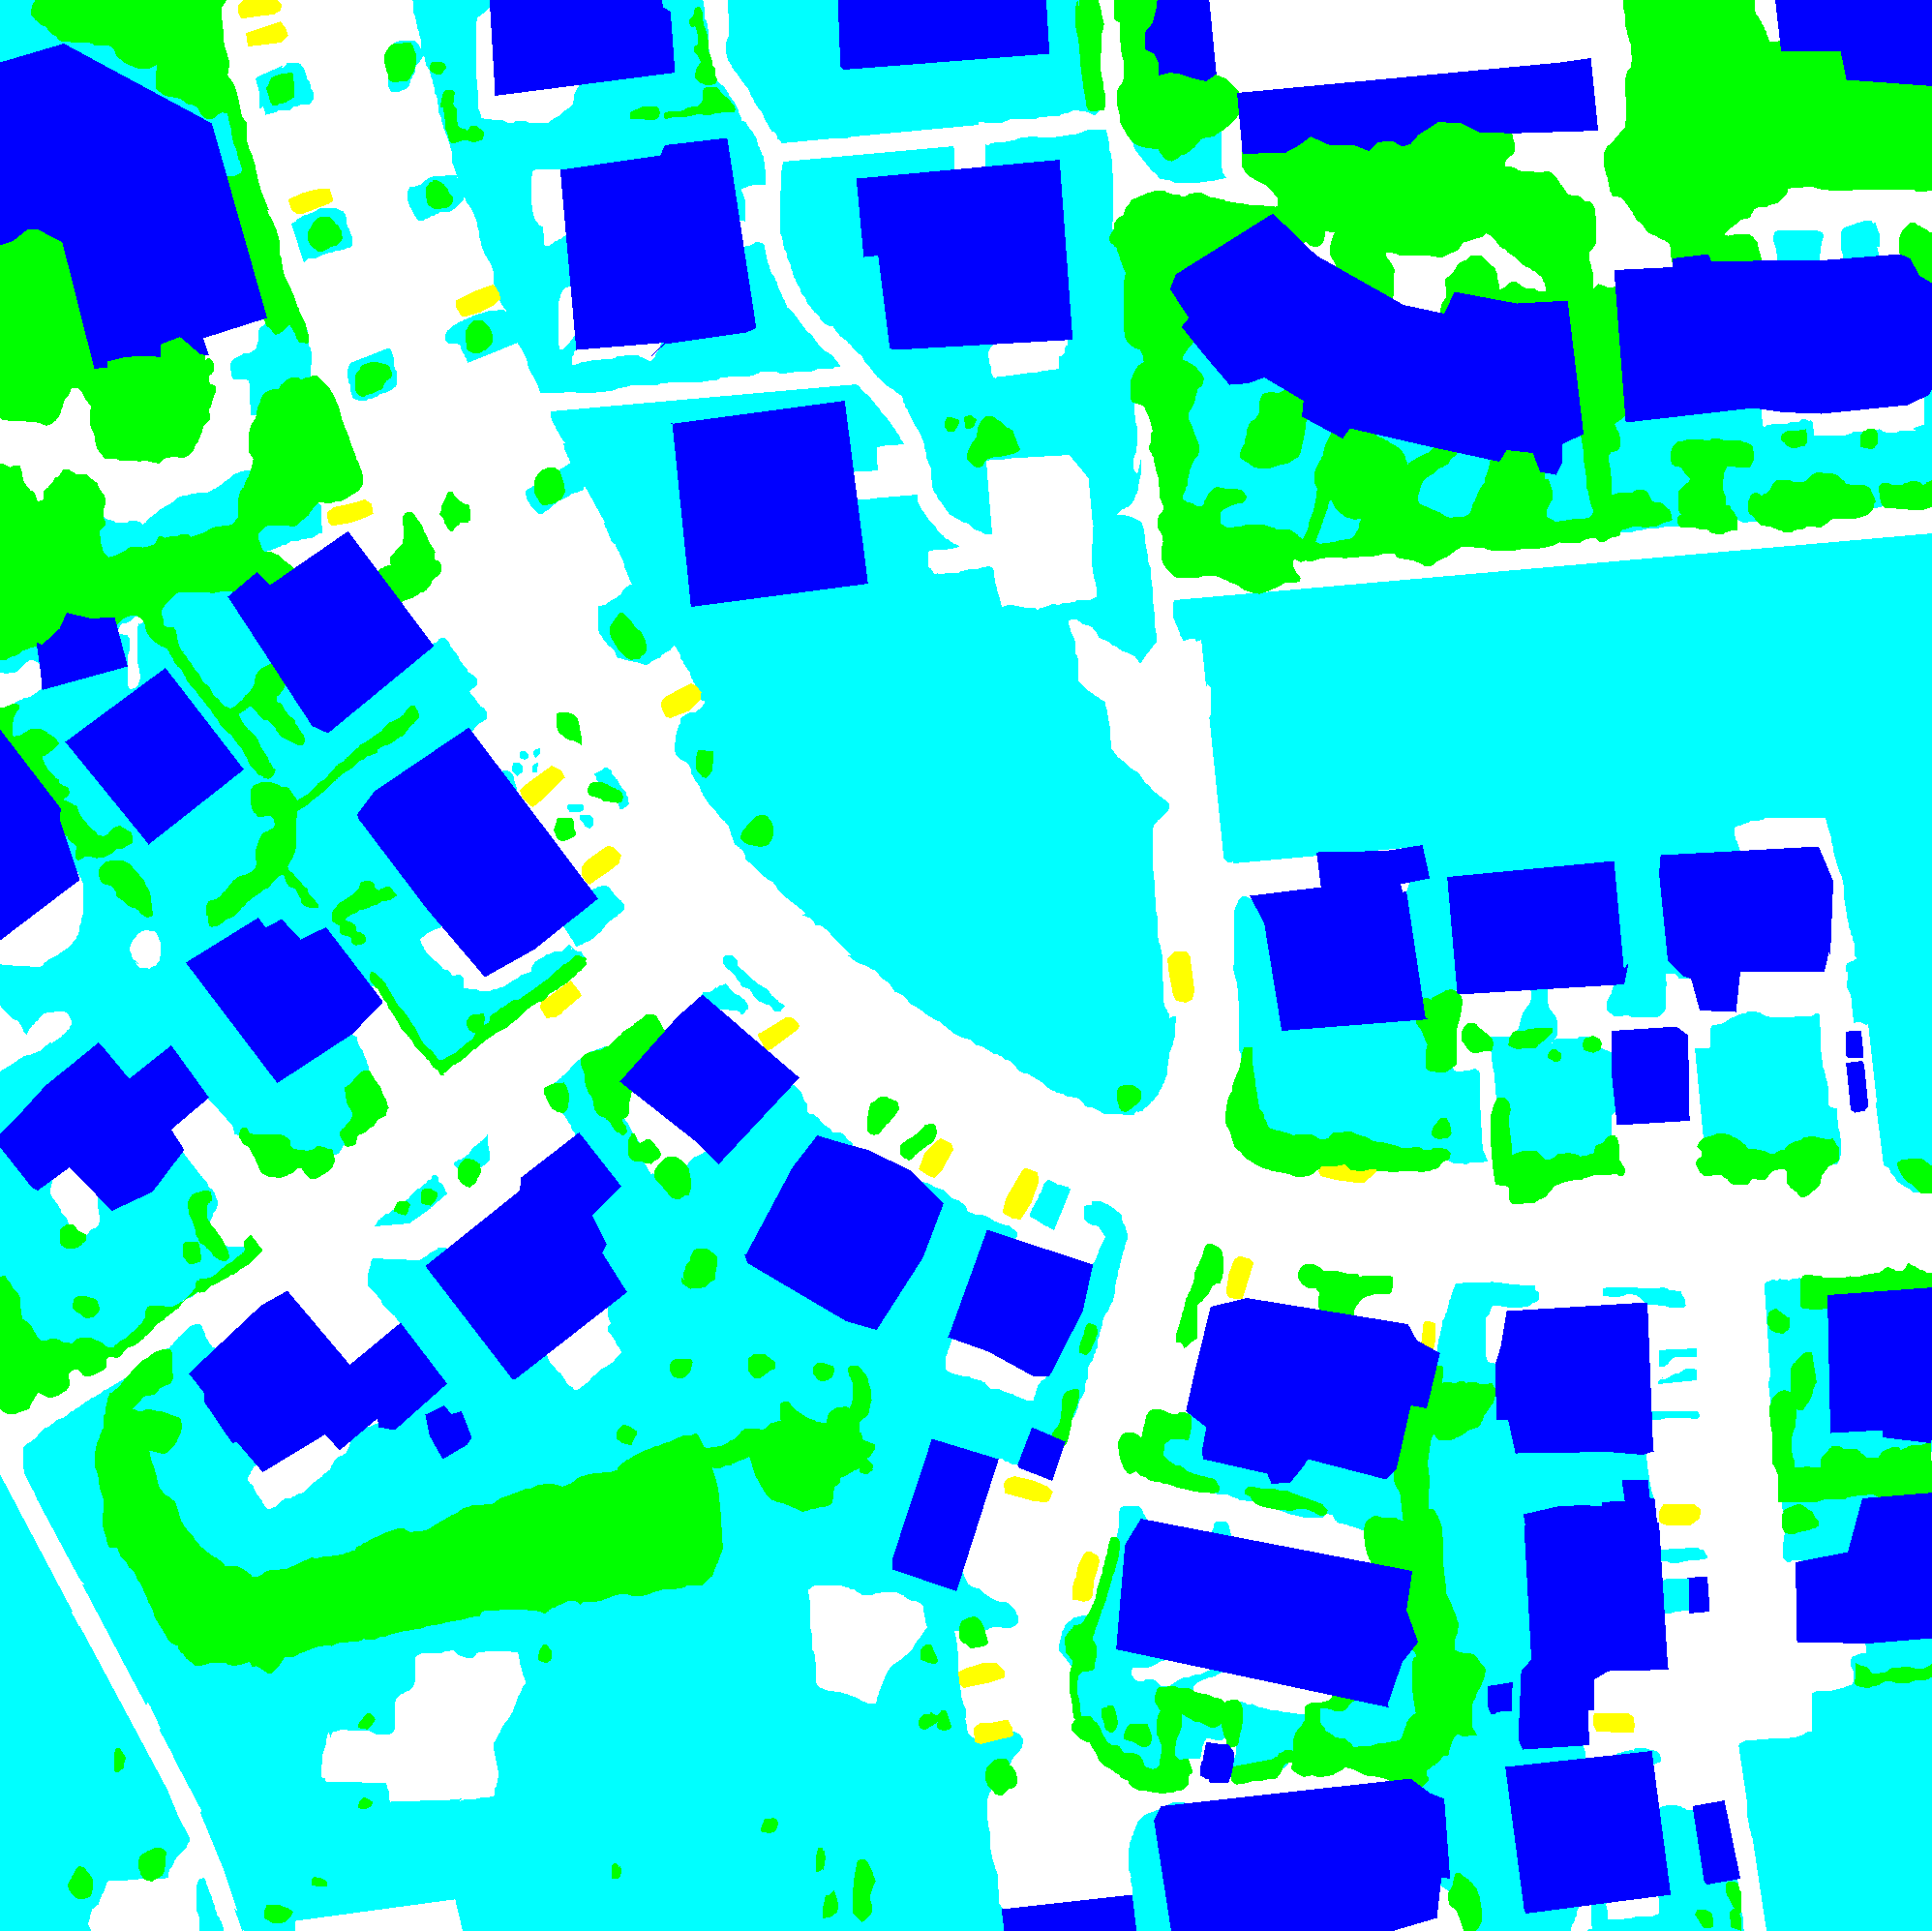
\includegraphics[width=11.5cm, height=7cm]{images/vaihingen-mask.png}
\centering
\caption{An mask From Vaihingen Dataset}
\label{fig:vaihingen-mask}
\end{figure}

\FloatBarrier
%%%LveDA%%%%%%%%it

The LoveDA dataset \cite{loveda} contains 5987 High Spatial Resolution (HSR )images with 166768 annotated pixels from three different cities in China. The images are obtained from Google Earth. The images are divided into two sub-categories: urban and rural. There are nine urban areas selected from different economically developed districts, which are all densely populated. The other nine rural areas were selected from undeveloped districts. The spatial resolution is 0.3 m, with
red, green, and blue bands. After geometric registration and pre-processing, each area is covered by 1024 × 1024 images, without overlap. LoveDA dataset contains a total of 7 classes: building, road, water, agriculture, barren, forest and background.

\FloatBarrier
\begin{figure}[ht]
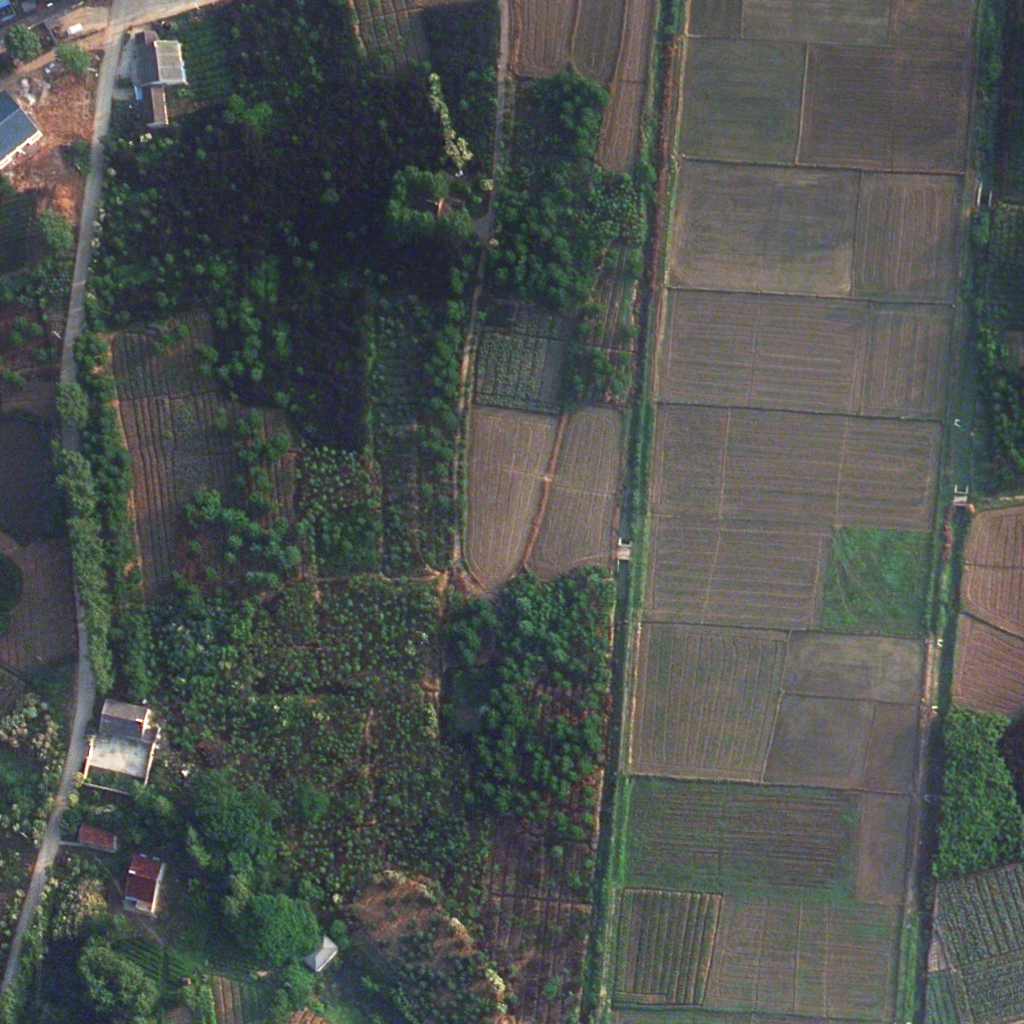
\includegraphics[width=11.5cm, height=7cm]{images/loveda-image.png}
\centering
\caption{An Image From LoveDa Dataset}
\label{fig:loveda-image}
\end{figure}

masukka mask

%%%%%%%GID%%%%%%%%%%%%
The GID-5 dataset \cite{GID2020} contains 120 6800 x 7200 HSR images with 5 classes. The classes are built-up, farmland, meadow, farmland and water which are pixel-level labeled with five different colors: red, green, cyan, yellow,
and blue, respectively. The images are obtained from Gaofen-2 satellite. GID-5 dataset is widely distributed over the geographic areas covering more than 50,000 $km^2$. Due to the extensive geographical distribution, GID-5 represents the distribution information of ground objects in different areas. Figure \ref{fig:gid-image} and \ref{fig:gid-mask} shows an example of an image and its corresponding mask from Deep Globe dataset.

\FloatBarrier
\begin{figure}[ht]
\includegraphics[width=11.5cm, height=7cm]{images/gid image.png}
\centering
\caption{An Image From GID-5 Dataset}
\label{fig:gid-image}
\end{figure}

\begin{figure}[ht]
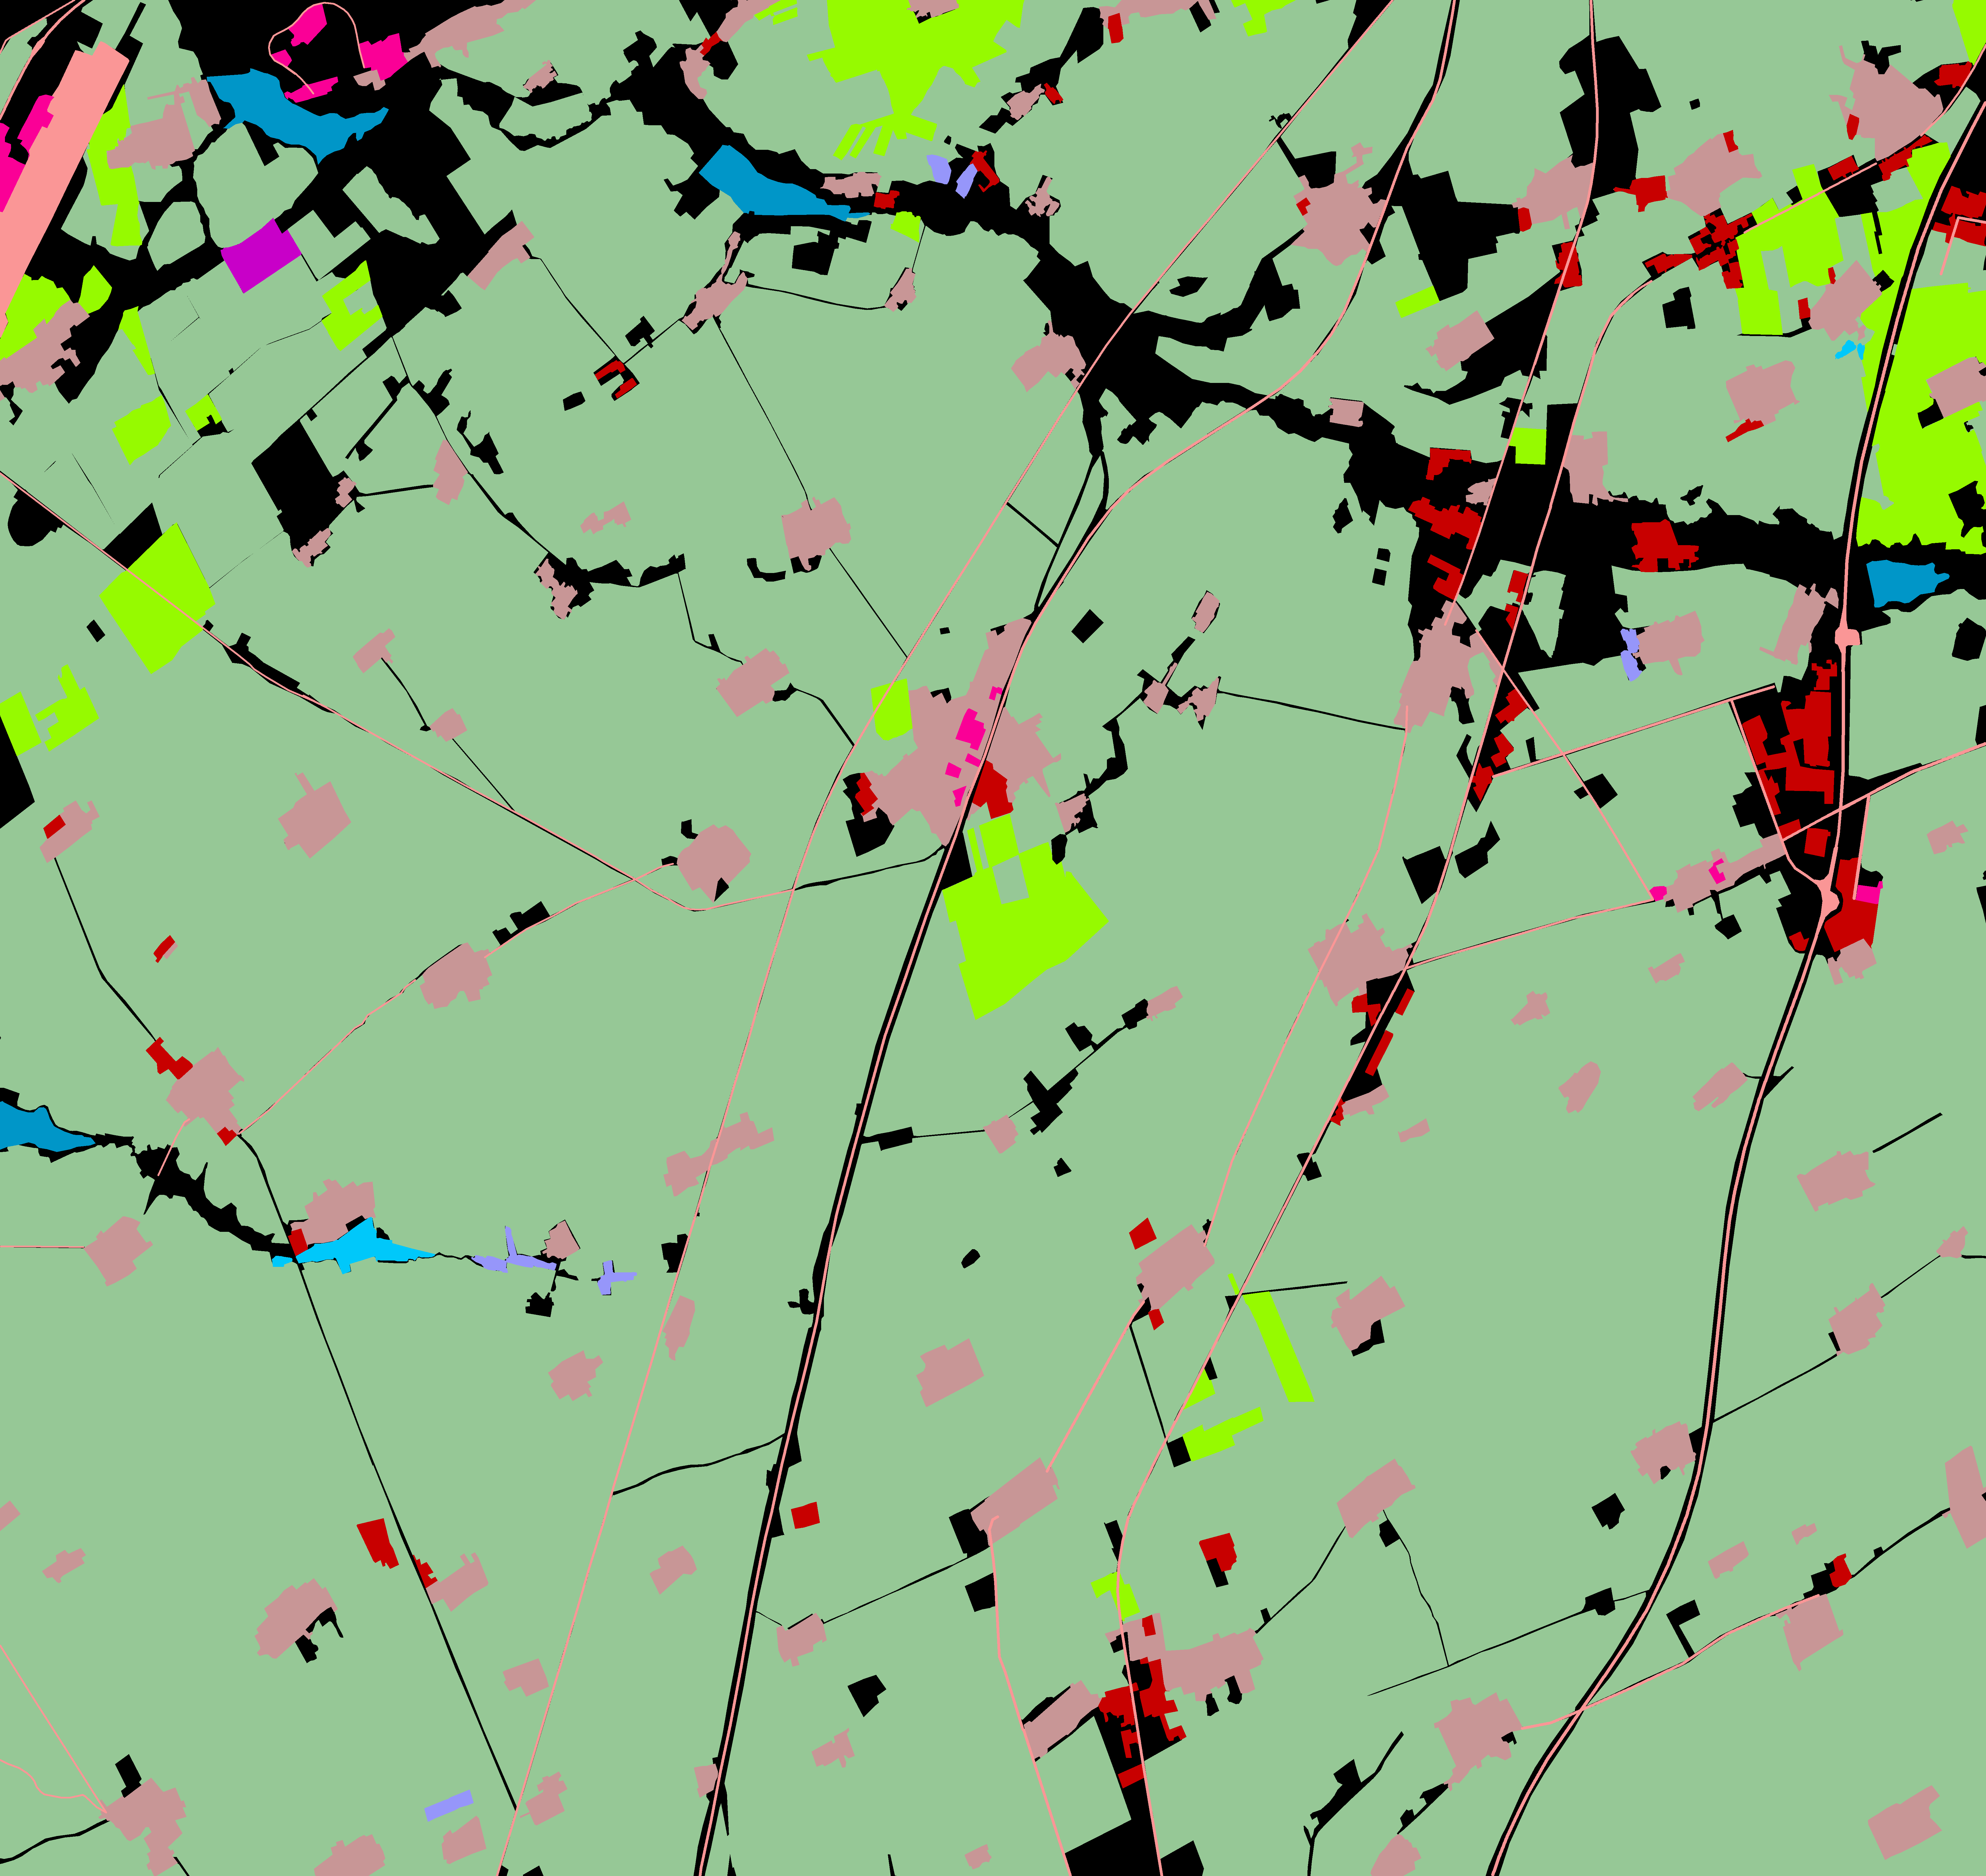
\includegraphics[width=11.5cm, height=7cm]{images/gid mask.png}
\centering
\caption{A Mask From GID-5 Dataset}
\label{fig:gid-mask}
\end{figure}
\FloatBarrier

%%deep-globe%%%
The Deep Globe Land Cover dataset \cite{deep-globe} contains 1146 satellite images of size 2448×
2448 pixels. The dataset is split into training, validation and test sets, each with 803/171/172 images. All images contain RGB channel, with a pixel resolution of 50 cm. The dataset is  collected from the DigitalGlobe Vivid+ dataset which is an earlier dataset containing satellite images. The annotations are pixel-wise segmentation masks created by professional annotators. There are 7 total classes:

\begin{enumerate}
    \item Urban land: Man-made, built up areas with human artifacts.
    \item Agriculture land: Farms, plantation, cropland, orchards, vineyards, nurseries, and ornamental horticultural areas; confined feeding infrastructure.
    \item Rangeland: Any non-forest, non-farm, green land, grass.
    \item Forest land: Any land with at least 20\% tree crown density plus clear cuts.
    \item Water: Rivers, oceans, lakes, wetland, ponds.
    \item Barren land: Mountain, rock, dessert, beach, land with no vegetation.
    \item Unknown: Clouds and others.
\end{enumerate}


Figure \ref{fig:deep-globe-image} and \ref{fig:deep-globe-mask} shows an example of an image and its corresponding mask from Deep Globe dataset.

\FloatBarrier
\begin{figure}[ht]
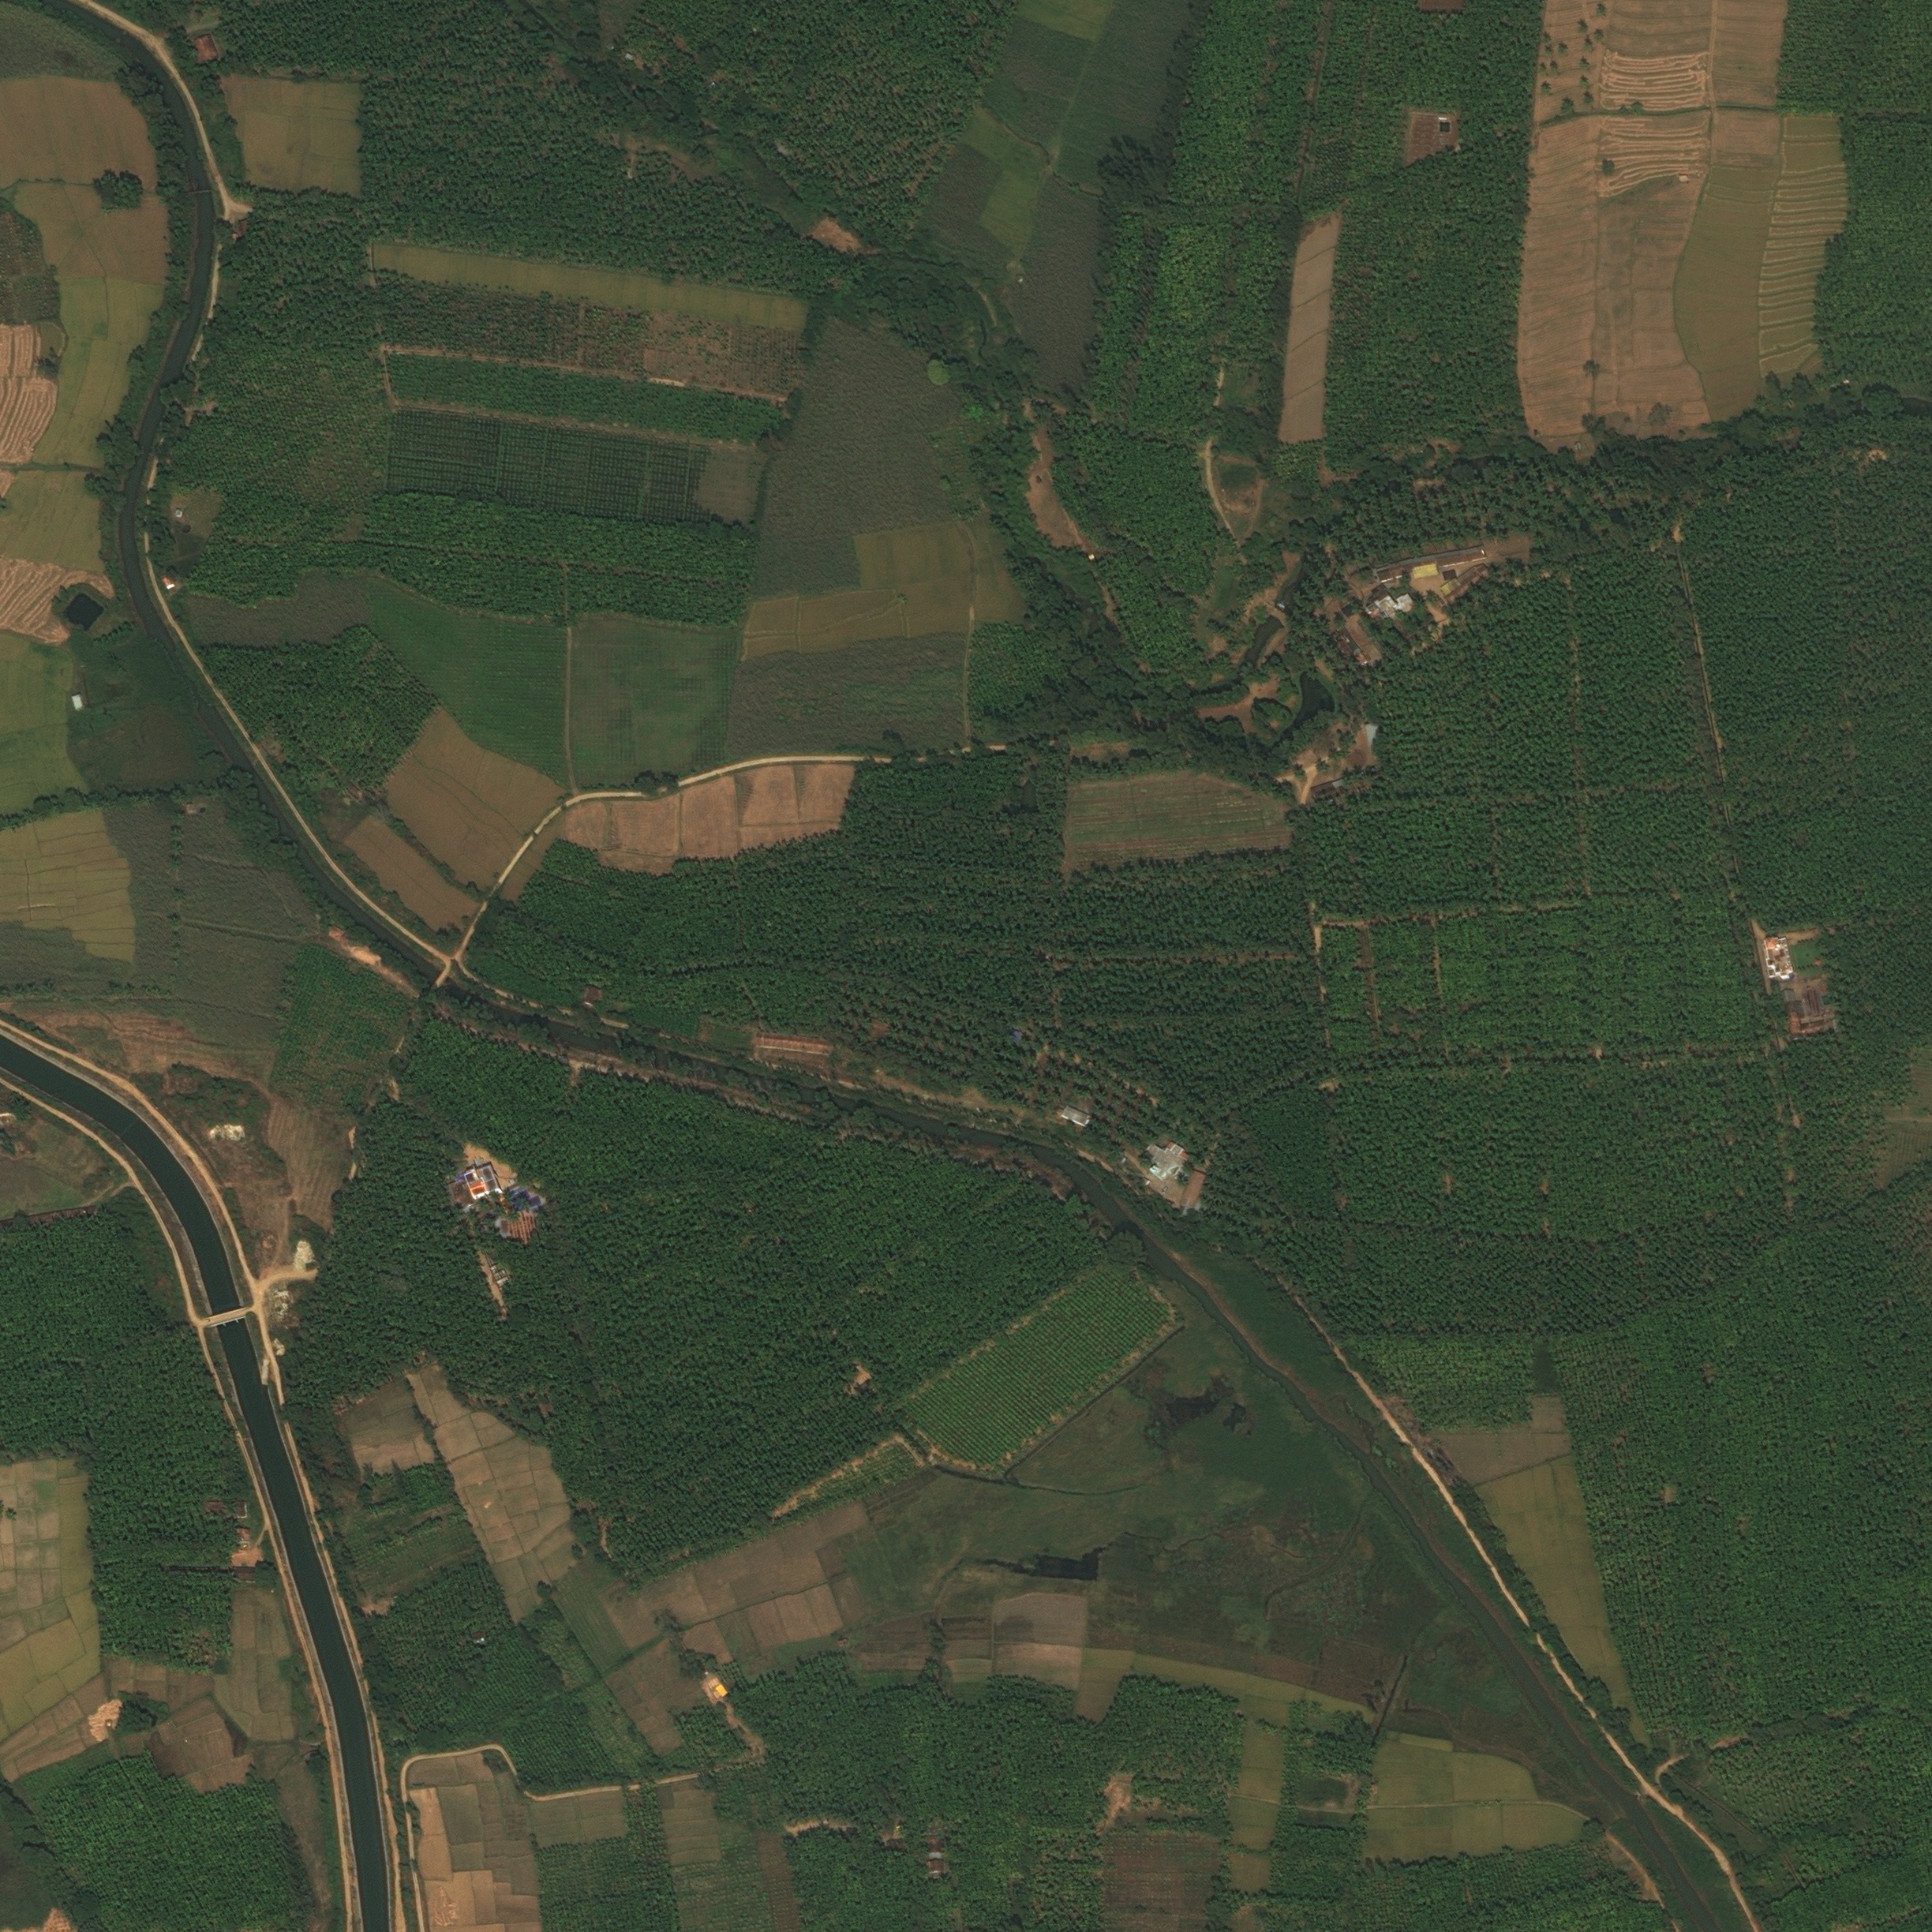
\includegraphics[width=11.5cm, height=7cm]{images/deepglobe_img.jpg}
\centering
\caption{An Image From Deep Globe Dataset}
\label{fig:deep-globe-image}
\end{figure}

\begin{figure}[ht]
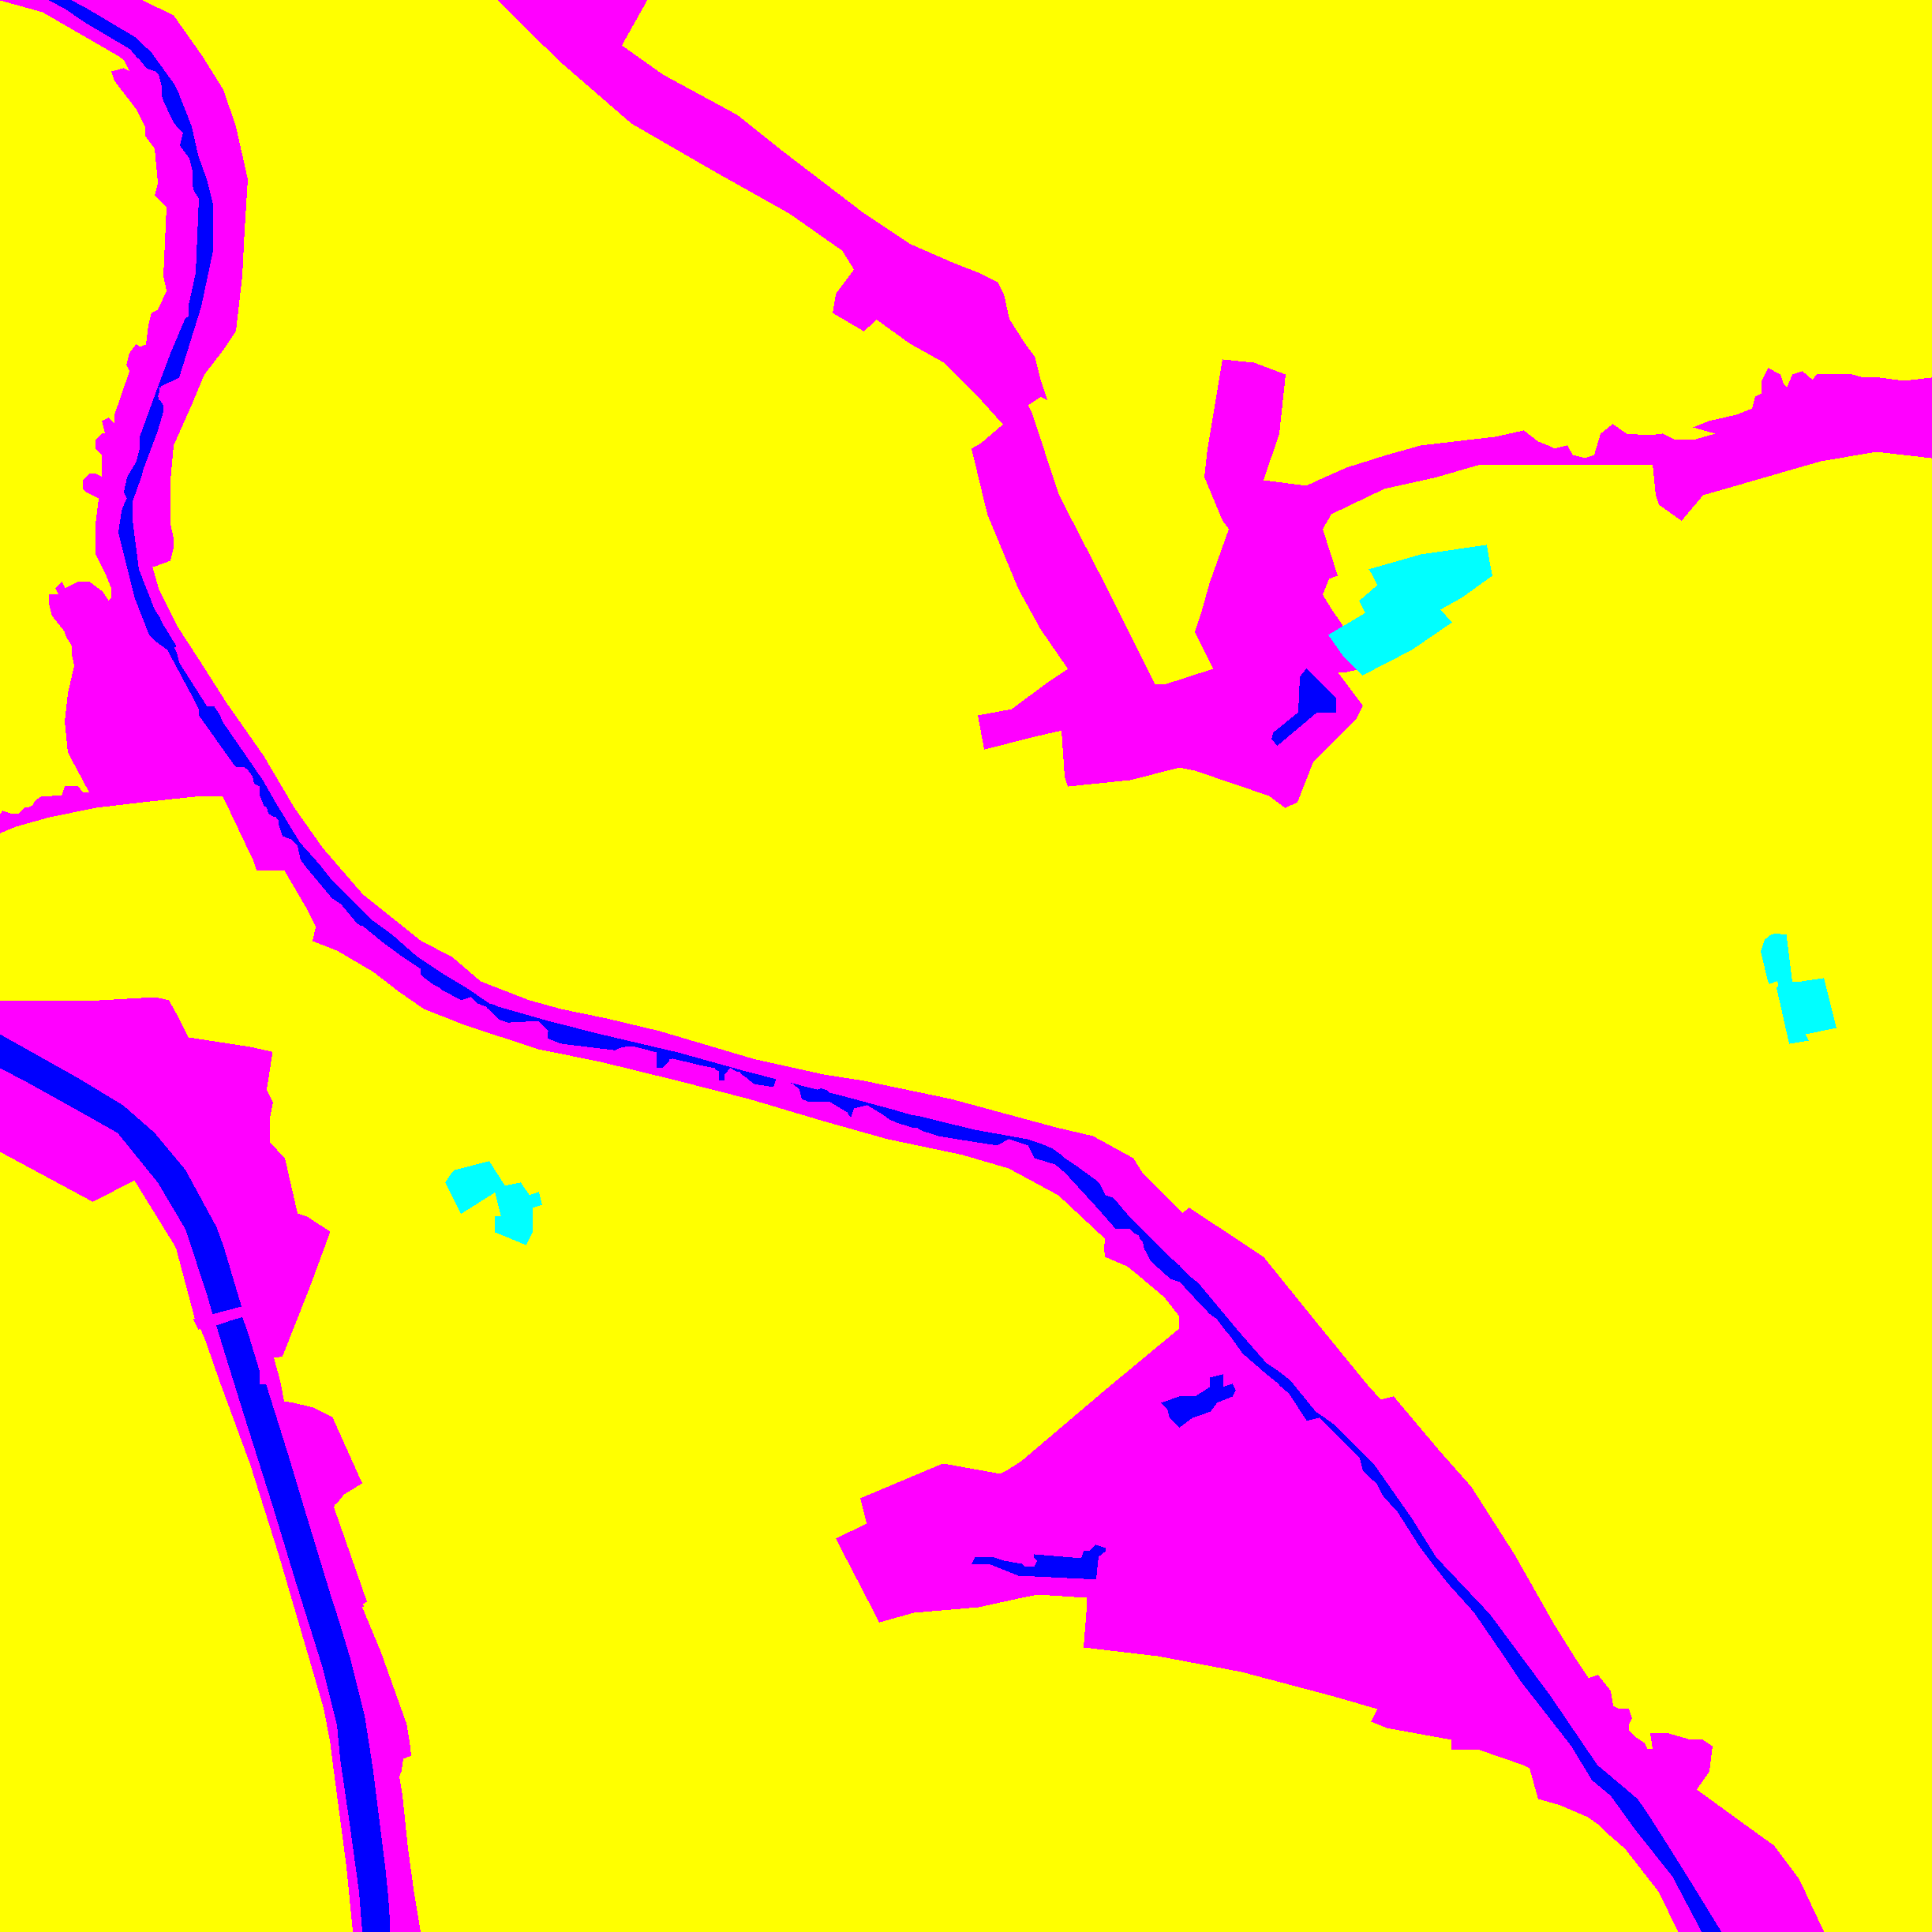
\includegraphics[width=11.5cm, height=7cm]{images/deepglobe_mask.png}
\centering
\caption{A Mask From Deep Globe Dataset}
\label{fig:deep-globe-mask}
\end{figure}
\FloatBarrier


The LandCover.ai dataset is a  simple RGB-only dataset with spatial resolution of 25 or 50 cm per pixel. There are 33 images with resolution 25 cm(9000 × 9500 px) and 8 images with resolution 50 cm (4200 × 4700 px). Pixel-wise annotations are made manually with VGG Image Annotator (VIA) by a group of people using polygon shape and polylines. LandCover.ai dataset has 5 classes: buildings, woodlands, water, roads and background.

masukkan landcover.ai


\section{Semantic Segmentation Before Deep Learning}

This section would elaborate on traditional methods of semantic segmentation, methods that do not apply any neural networks but make heavy use of domain knowledge and feature extraction methods. 

\subsection{Feature Extraction}
Before we apply any of the classification method that will be discussed in the proceeding sections (SVM, Random Decision Forest, MRF, CRF) we must extract the features from an image. The accuracy of traditional semantic segmentation methods heavily depends on the selected features. The features may be the numerical value of each pixel or the feature map containing the gradient of each pixel. There are three feature extraction methods discussed in this section, namely they are Histogram of Oriented Gradients, Scale-Invariant Feature Transform and Bag of Visual Words .

\begin{enumerate}
    \item \textbf{\textit{Histogram of Oriented Gradients (HOG).}} HOG features interpret any given image as a discrete function $I : \mathbb{N}^2 \rightarrow \{0...255\}$ that maps a pair value $(x,y)$ which is the coordinate of the pixel to an RGB value. Then, the partial derivative in of \(x\) and \(y\) are calculated for every pixel. The input image is now transformed into a feature map with the gradient of each pixel. Lastly, the constructed feature map is divided into smaller patches and the direction and magnitude of the histogram is calculated for each patch. \cite{DBLP:journals/corr/Thoma16a}.

    \begin{figure}[ht]
    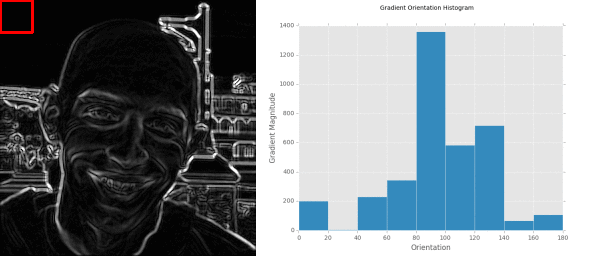
\includegraphics[width=12cm, height=6cm]{images/hog.png}
    \centering
    \caption{Computing a histogram of oriented gradients for the first patch of an input image.}
    \label{fig:hog}
    \end{figure}
    
    \item \textbf{\textit{Scale-Invariant Feature Transform (SIFT).}} SIFT is a feature extraction algorithm that was introduced in 2004. Unlike HOG, SIFT is not affected by the orientation or scale of the input image. \cite{DBLP:journals/corr/Thoma16a}. An image will be divided into smaller patches and the difference-of-Gaussian (DoG)is calculated. DoG is obtained as the difference of Gaussian blurring of an image with two different $\sigma$. Next, local extrema is searched to be be assigned as potential key points. Lastly, after the key points are discovered, an 8-bin orientation histogram is created for each patch to math the key points. The final output will be a feature map containing accepted key points. A more thorough explanation is available in the original paper \cite{SIFT}.

    \begin{figure}[ht]
    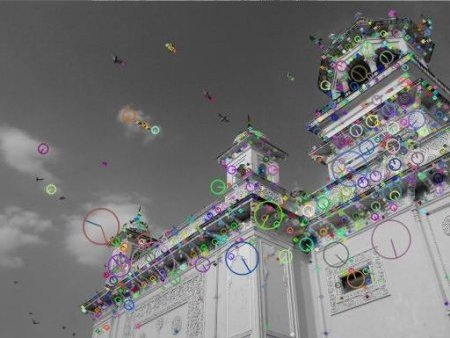
\includegraphics[width=12cm, height=7.5cm]{images/sift_keypoints.jpg}
    \centering
    \caption{Each circle represents the location and orientation of SIFT keypoints}
    \label{fig:sift_keypoints}
    \end{figure}

    
    \item \textbf{\textit{Bag of Visual Words (BOV).}} BOV construct sparse histograms that contain the frequency of features in an image. Those features are usually extracted using SIFT \cite{DBLP:journals/corr/Thoma16a}. BOV is often used alongside other feature extractors such as SIFT by assigning each SIFT descriptor to the closest entry in a visual dictionary.
\end{enumerate}

\subsection{Random Decision Forest for Semantic Segmentation}
 A decision tree is a tree where each leaf represents a class and each non-leaf nodes uses the feature inputs to decide which branch to descend to \cite{DBLP:journals/corr/Thoma16a}. A random decision tree is as decision tree that is injected with some randomness during the training phase  to reduce over-fitting and increase accuracy. Random Decision Forest is an unsupervised ensemble learning method that are made up of multiple independently constructed random decision trees. An in-depth explanation to semantic segmentation using Random Decision Forest is given by \cite{Schroff2008ObjectCS}. 
 
\subsection{Support Vector Machines (SVM) for Semantic Segmentation}

In SVM the training data is represented as $(x_i,y_i)$ where $x_i$ is the feature vector, $y_i \in \{-1,1\}$ is the class label and $i \in \{1...m\}$ where m is the number of inputs.

Assuming that the data is linearly separable, SVM is a task of solving the optimal margin classifier:

\begin{equation*}
    min_{w,b} \quad \frac{1}{2}||w||^2 \\
\end{equation*}

\begin{equation*}
    s.t. \quad y^{i}(w^T x^i +b)\geqslant 1, i \in {1...m}
\end{equation*}

\vspace{0.1cm}

\noindent $w$ is the linear combination of the training data $x$:

\begin{equation*}
    w = \sum_{i=1}^m \alpha_i y_i x_i
\end{equation*}

\noindent Where $\alpha$ is the Lagrange multiplier. Not every dataset is linearly separable thus this problem can be solved by transforming the feature vectors $x$ into a higher dimension using a non-linear mapping $/psi$. Thus instead of learning using $x$, we may learn using a higher-dimensional features $\psi(x)$, this method is called the \textit{kernel trick}. Specifically, given a feature mapping $\psi$, we define the corresponding kernel to be:    

\begin{equation*}
    K(x,z)=\psi(x)^T\psi(z)
\end{equation*}

The SVM described above can only distinguish between binary classes.The one-vs-all strategy and the one-vs-one strategy are methods used to expand it to be a multi-class classifier.. In the one-vs-all strategy n classifiers have to be trained which can distinguish one of the n classes against all other classes. In the one-vs-one strategy $\frac{n^2-n}{2}$ classifiers are trained; one classifier for each pair of classes.

\subsection{Markov Random Field (MRF)} MRF maps an image onto an undirected graph where each node is a pair of random variable $(x,y)$ assigned to each pixel and the edges connect adjacent pixels \cite{YU201882}. $x$ represents the class label of a pixel and $y$ represents the RGB value of a pixel. Which means $x$ has a range of ${0...n}$ and y has a range of ${0...255}$ with $n$ being the number of classes.  Every edge is assigned conditional dependencies of its connecting nodes as weight. The probability of $x,y$ can be expressed as:

\begin{equation*}
    P(x,y) = \frac{1}{Z} e^{-E(x,y)
\end{equation*}

\noindent where $Z = \sum_{x,y}e^{-E(x,y)}$ and it is called the partition function whereas E is called the energy function. A commonly used energy function is $E(x,y) = \sum_{c\in C}\psi_{c}(x,y)$, where $\psi$ is called the clique potential \cite{DBLP:journals/corr/Thoma16a}. A thorough presentation of MRF can be found in \cite{markovbook}. 

\subsection{Conditional Random Field (CRF) for Semantic Segmentation} CRF is an extension of MRF. Instead of learning the distribution $P(x,y)$, it chooses to learn $P(x|y)$ \cite{DBLP:journals/corr/Thoma16a}. There are two advantages that CRF has over MRF. The first one being it does not to estimate the distribution of x. The second advantage is the consequence of the first one, as the distribution of x is not being estimated, less computation is required hence making CRF faster than MRF \cite{YU201882}. CRF has the partition function $Z(x)$:
\begin{equation*}
    Z(x) = \sum_{x} P(x,y)
\end{equation*}

\noindent and the joint probability distribution is given as follows:

\begin{equation*}
    P(y|x) = \frac{1}{Z(x)} \prod_{c \in C}\psi_{c}(y_{c}|x)
\end{equation*}

\noindent CRF is often used in conjunction with neural networks as a post-processing method for semantic segmentation task. It is is used to smoothen the output mask \cite{crf-semantic}.

\section{Limitations of Traditional Methods}
\begin{enumerate}
    \item The traditional method is simply less accurate. As an example the best traditional method back in 2015 which utilized SIFT features extraction method and Fisher Vectors, had a performance of about 25.7\% error rate on semantic segmentation task on ILSVRC-2010 dataset. While AlexNet proposed by \cite{alexnet} had an error rate of 17.0\% \cite{DBLP:journals/corr/Thoma16a}.
    \item  Feature extraction method such as SIFT and Random Decision Forest require researchers to come up with a good hand-crafted feature to achieve high accuracy while good features are very hard to produce. Compared this with the automatically learned features provided by deep learning, traditional methods would require a lot more time and effort.

\end{enumerate}

\section{Semantic Segmentation of Satellite Images Using Convolutional Neural Networks}

Semantic segmentation task has been long dominated by Convolutional Neural network (CNN). The Fully Convolutional Network (FCN) \cite{7298965} is the first network proven to be an effective method to extract features automatically and serves as an effective end-to-end CNN structure for semantic segmentation task. The outcome of FCN, although encouraging, appears to be coarse due to the over-simplified design of the decoder.

To tackle this problem, better CNNs were proposed such as U-Net \cite{unet} which  introduced the encoder-decoder framework. Since its introduction, the encoder-decoder framework has become the standard structure of satellite images segmentation network \cite{unetformer}. U-Net introduced two symmetric paths: a contracting path, which is also known as the encoder to extract local features, and an expanding path which is also called the decoder, for extracting position. The encoder gradually apply convolutions and max pooling to reduce the resolution of the feature map, while the decoder extracts contextual information by progressively restoring the spatial resolution. At every level of the decoder skip connections are used to by concatenate the output of the decoder with the feature maps from the encoder. Figure \ref{fig:unet} show the U-Net architecture. Benefiting from its translation equivariance and locality, U-Net enhances the semantic segmentation performance significantly and the encode-decoder framework has been a major influence towards semantic segmentation task. 

\begin{figure}[ht]
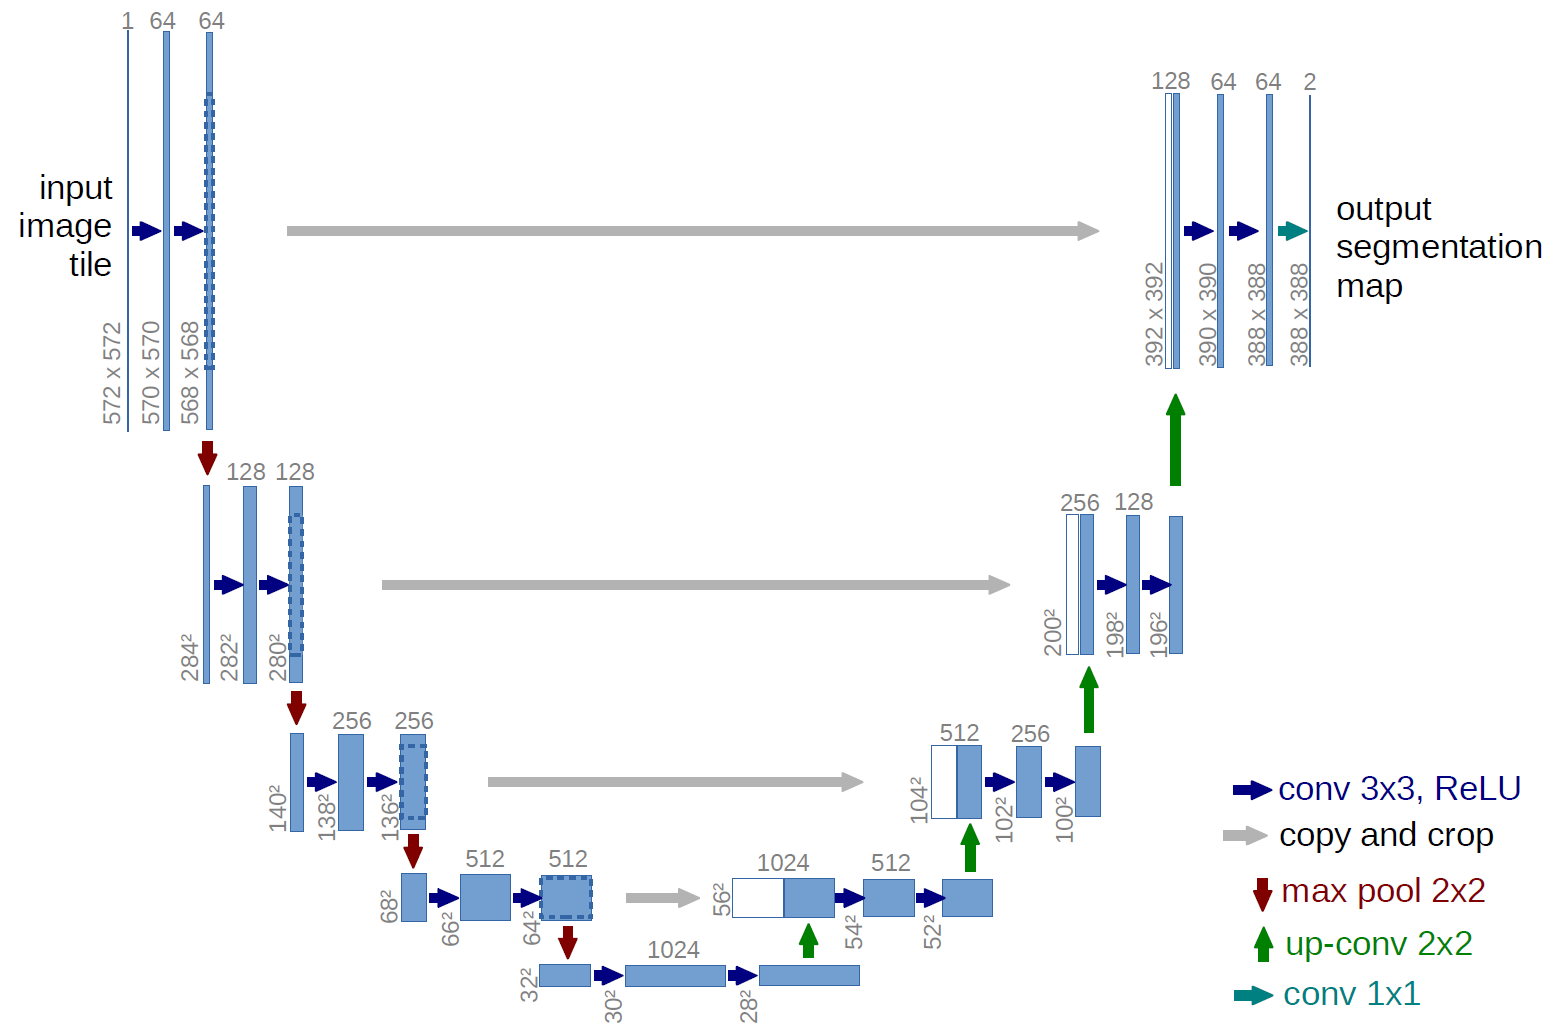
\includegraphics[width=10.5cm, height=7cm]{images/unet.png}
\centering
\caption{U-Net Architecture}
\label{fig:unet}
\end{figure}

Even though the results are promising, the long-range dependency of U-Net is limited by the locality property of the convolutional mechanism, which is critical for semantic segmentation. There are two types of approaches to address this issue, either modifying the convolution operation or utilizing the attention mechanism. Such examples of the first approach is to enlarge the receptive fields using large kernel sizes \cite{enlarge-receptive-field}, or utilising feature pyramids \cite{feature-pyramid}. On the other hand the second approach focuses on integrating attention mechanisms with the encoder-decoder architecture to capture long-range dependencies of the feature maps, examples can be found in Attentive Bilateral Contextual Network \cite{abcnet} and Attention U-Net \cite{attention-unet}. Although the second approach showed better performance, both approaches failed to decouple the network from the dependence of the encoder-decoder structure. In the context of semantic segmentation, per-pixel classification is often inaccurate if only local information is taken into account \cite{swin-v1}.

Attention U-Net \cite{attention-unet} is a model that aims to improve U-Net by introducing attention gates in the skip connections between the encoder and decoder as shown in \ref{fig:attention-unet}. The results showed that Attention U-Net performs better than traditional U-Net for segmentation of CT scans images.

\begin{figure}[ht]
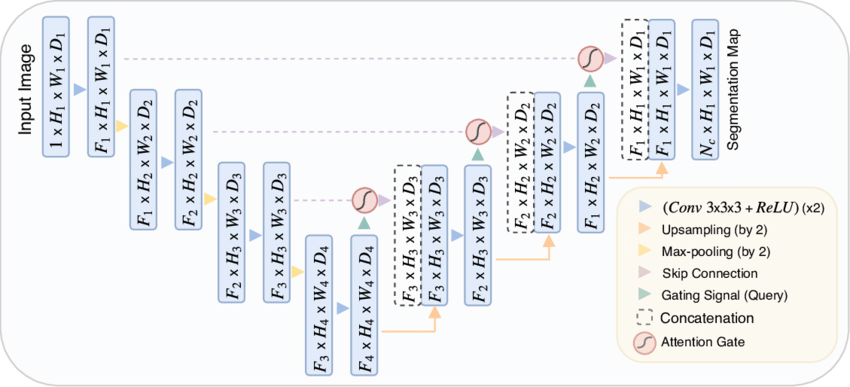
\includegraphics[width=10.5cm, height=7cm]{images/attention-unet.png}
\centering
\caption{Attention U-Net Architecture}
\label{fig:attention-unet}
\end{figure}

U-Net with added attention mechanism is the approach favored by most literature focusing on semantic segmentation of satellite images. Multi Attention U-Net(MA-Unet) \cite{multi-attention-unet}  uses residual structure and simple attention modules. According to figure \ref{fig:maunet} the decoder in MA-Unet uses transposed convolution and attention modules at every feature fusion stage. MAUnet performed semantic segmentation task on the WHDLD datasets and DLRSD datasets. WDLD dataset have 8 classes while DLRSD dataset have 17 classes covering common classes such as farms, grasslands and lakes. MA-Unet was compareed with other U-Net based models susch as U-Net, U-Net++, Attention U-Net and MagNet on the same task. MA-Unet performs better at segmenting classes with fine details such aeroplanes. MA-Unet has the highest mIOU on both dataset with 63.94\% on WHDLD and 61.90\% on DLRSD.

Spatial Attention U-Net (SA-Unet) \cite{improved-unet} uses atrous spatial pyramid pooling as its encoder and attention modules at every skip connection like we have seen in Attention U-Net.  \cite{attention-unet-road} employs U-Net with attention to extract roads from satellite images. Instead of using simple attention modules at every skip connections, they uses attention module only once at the lowest skip connection.

\begin{figure}[ht]
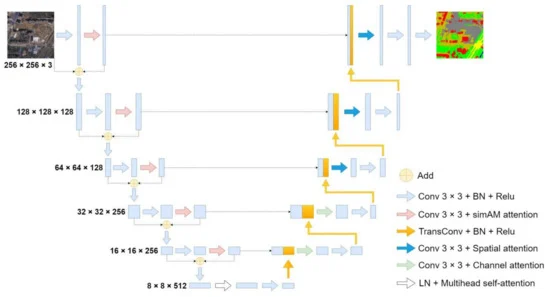
\includegraphics[width=10.5cm, height=7cm]{images/maunet.png}
\centering
\caption{Multi Attention U-Net Architecture}
\label{fig:maunet}
\end{figure}

\section{Semantic Segmentation of Satellite Images Using Vision Transformers}

Transformers were introduced by \cite{attention-is-all-you-need} and since its inception it has been the de facto model for Natural Language Processing (NLP). Transformers that are used for image processing are called Vision Transformers to differentiate it from its NLP counterpart. Vision Transformers essentially translates 2D image-based tasks into 1D sequence-based tasks.





\section{Advantages of Vision Transformer for Semantic Segmentation of Satellite Images}
\begin{enumerate}
    \item \textit{\textbf{General Modelling Capability}}
    
    There are two aspects that gives a vision transformer general modelling capabilities. The first one being performing a task using a transformer can be interpreted as working on a fully connected graph. Any concept, can be represented by the nodes in a graph, and the relationship between concepts are represented by the graph edges.

    Every task in computer vision deals with processing two basic granular elements: pixels and objects. Thus, there are three type of relationship that can be found: pixel-to-pixel, object-to-object and pixel-to-object. The transformer's attention mechanism allows researchers to include all 3 types of relationships in one network. For examples, networks such as DETR \cite{detr}, LearnRegionFeat \cite{learnregionfeat} and RelationNet++ \cite{regionnet++} model the relationship between object and pixel to achieve SOTA performance in semantic segmentation task.  

    \item \textit{\textbf{Attention Mechanism Complements Convolution}}

    Unlike convolution which is a local operation, the attention mechanism is a global one which means it can model the relationship between all the pixels in an image. This two layers complement each other very well and works such as DETR \cite{detr} and Swin Transformer V2 \cite{swin-v2} are evidence of this claim.

    \item \textit{\textbf{Transformers are Scalable}}

    Transformers has shown excellent scalability in Natural Language Processing. However, when transformers were initially used for computer vision, a lot of researchers doubted it ability to scale because all of the networks are dense as it has to process every pixel as input. Fortunately, there are recent works that shows we can improve the scalability of transformer by increasing its efficiency and reducing its computational load. Vision MoE from Google managed to match the performance of SOTA networks, while slashing the compute time into half by using a sparse network. It managed to train a 15 billions parameter model with 90.35\% accuracy on ImageNet dataset \cite{scaling-sparse}. Figure \ref{fig:scaling} shows the recorded number of parameters in Vision Transformer models from 2018 until 2022

\begin{figure}[ht]
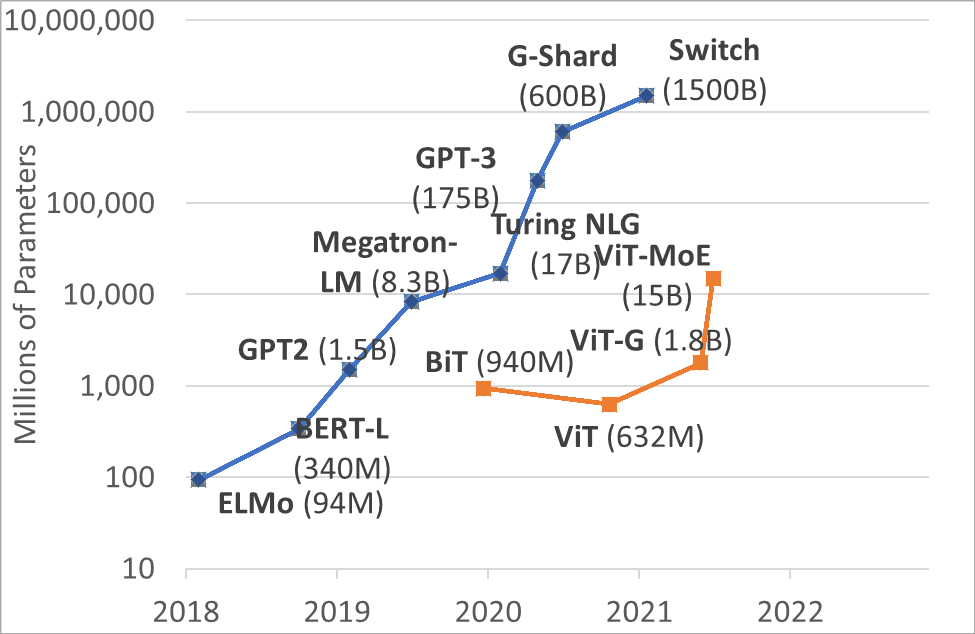
\includegraphics[width=10cm, height=6.5cm]{images/scaling.png}
\centering
\caption{The size records of vision transformer in recent years}
\label{fig:scaling}
\end{figure}
\end{enumerate}
